We studied how varying the temporal and spatial resolution modifies the behavior of the thermohaline zone that develops between the burning shell and the convective envelop, and the results of these tests are summarized in TODO.
For the suite of simulations presented in this paper, we increased the spatial and temporal resolution of our simulations by using a mesh delta coefficient of 0.8 and time delta coefficient of 0.5 for most of the star's evolution.
After the main sequence once we measured $log g < 3$, we decreased the mesh delta coefficient to 0.5 and the time delta coefficient to 0.1; we found that this combination of temporal and spatial resolution produced high accuracy at reasonable computational cost.


\begin{figure*}[!tb]
\begin{center}
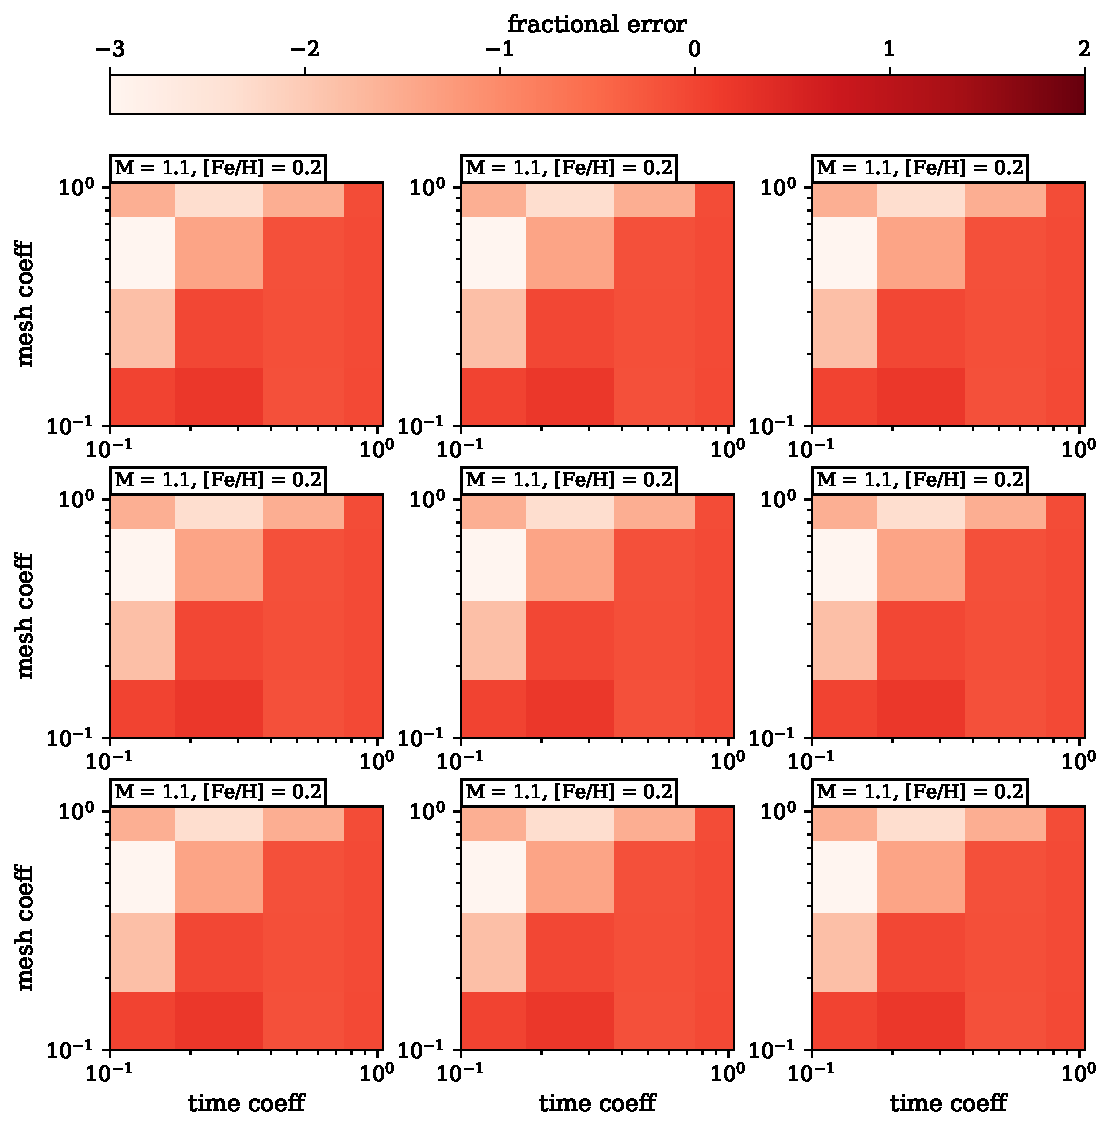
\includegraphics[width=\textwidth]{./figures/resolution_test/resolution_test.pdf}
\caption{This is a template figure showing relative error in a calculation as a function of mesh and time delta coefficient. It'll look nicer. }
\label{Fig:resolution_test}
\end{center}
\end{figure*}